% !TEX root = ../algo-summary.tex

\section{Network Flow}\label{sec:network_flow}

restricted version of a more general optimization problem, called linear programming.

\begin{definition}[Flow Network]\label{def:flow_network}
Abstraction for stuff \emph{flowing} through the edges of a network.
A flow network is a directed graph \(G = (V, E)\) with a \emph{source} and a \emph{sink} node \(s, t \in V\) (where flow originates and is consumed, respectively),
Each edge \((u,v) \in E\) has a capacity \(c(u,v) \in \N_0\), where \(c(u,v) = 0\) if \((u,v) \notin E\).
\end{definition}

\begin{remark}
Multiple sources/sinks can be modeled by adding a \emph{super-source} and \emph{super-sink} with infinite capacity.
\end{remark}

\begin{caution}
If we have further restrictions, such as flow from certain sources can only go to certain sinks, we have the \emph{multi-commodity flow problem}, which is NP-hard.
\end{caution}

\subsection{Maximum Flow and Minimum Cut}\label{sec:max_flow_min_cut}

Two rich algorithmic problems with a beautiful duality. 
Cornerstones in combinatorial optimization.


\begin{definition}[Flow]\label{def:flow}
A \emph{\(s\)-\(t\) flow} is a function \(f : E \to \R_{\ge 0}\) that satisfies
\begin{itemize}
  \item \emph{Capacity:} For each \(e \in E\)
  \begin{equation}\label{eq:capacity_constraints}
    0 \le f(e) \le c(e)
  \end{equation}
  \item \emph{Conservation:} For each \(v \in V \setminus \{s,t\}\)
  \begin{equation}\label{eq:flow_conservation}
    \sum_{u \in V} f(u,v) = \sum_{w \in V} f(v,w)
  \end{equation}
\end{itemize}
where \(s, t \in V\) are the source and sink nodes.
\end{definition}
\begin{definition}\label{def:flow_value}
The \emph{value} \(v(f)\) (also denoted by \(|f|\)) of a flow \(f\) is
\begin{equation}\label{eq:flow_value}
  {\color{Red}\boxed{\color{black}
  v(f) \coloneqq \sum_{w \in V} f(s,w) = \sum_{u \in V} f(u,t)
  }}
\end{equation}
where equality follows from flow conservation.
\end{definition}

\begin{problem}[Max Flow]\label{prob:max_flow}
Find an \(s\)-\(t\) flow \(f\) of maximum value \eqref{eq:flow_value}.
\end{problem}

% \begin{remark}
% If all capacities \(c(u,v)\) are integers, there always exists a maximum flow \(f\) such that all \(f(u,v)\) are integers.
% \end{remark}




\begin{definition}\label{def:cut}
An \emph{\(s\)-\(t\) cut} is a partition \((A,B)\) of \(V\) with \(s \in A\) and \(t \in B = V \setminus A\).
\end{definition}
\begin{definition}
[Cut Capacity]
\label{def:cut_capacity}
The \emph{capacity} of the cut is
  \begin{equation}\label{eq:cut_capacity}
  {\color{Red}\boxed{\color{black}
    c(A,B) \coloneqq \sum_{a \in A} \sum_{b \in B} c(a,b)
  }}  
  \end{equation}
i.e. the summation of all edges going from \(A\) to \(B\).
\end{definition}

\begin{problem}[Min Cut]\label{prob:min_cut}
Find an \(s\)-\(t\) cut \((A,B)\) of minimum capacity \eqref{eq:cut_capacity}.
\end{problem}





\begin{definition}\label{def:cut_flow}
The \emph{net flow} across the cut is
  \begin{equation}\label{eq:cut_flow}
  {\color{Red}\boxed{\color{black}
  f(A,B)
  \coloneqq 
  % \sum_{u \in A, v \in B} f(u,v) - \sum_{u \in B, v \in A} f(u,v) 
  \sum_{u \in A} \sum_{v \in B} f(u,v) - \sum_{u \in B} \sum_{v \in A} f(u,v)
  }}
  \qedhere
  \end{equation}
\end{definition}



\begin{lemma}[Flow Value]\label{lem:flow_value}
Let \(f\) be any flow and \((A,B)\) be any cut. Then
\begin{equation}\label{eq:flow_value_cut}
  f(A,B)
  = 
  v(f)
\end{equation}
i.e. the net flow across the cut equals the value of the flow.
\end{lemma}
\begin{proof}
\[
\begin{verticalhack}
\begin{aligned}
  v(f) &\overset{\text{\eqref{eq:flow_value}}}{=} \sum_{v \in V} f(s,v) \\
       &=\sum_{v \in V} f(s,v) + 0 \\
       &\overset{\text{\eqref{eq:flow_conservation}}}{=} \sum_{v \in V} f(s,v) + \sum_{u \in A \setminus \{s\}} \left( \sum_{v \in V} f(u,v) - \sum_{v \in V} f(v,u) \right) \\
        &= \sum_{u \in A} \left( \sum_{v \in V} f(u,v) - \sum_{v \in V} f(v,u) \right) \\
       &= \sum_{u \in A} \sum_{v \in V} f(u,v) - \sum_{u \in A} \sum_{v \in V} f(v,u) \\
        &= \sum_{u \in A} \left( \sum_{v \in A} f(u,v) + \sum_{v \in B} f(u,v) \right) - \sum_{u \in A} \left( \sum_{v \in A} f(v,u) + \sum_{v \in B} f(v,u) \right) \\
        &= \cancel{\sum_{u \in A} \sum_{v \in A} f(u,v)} + \sum_{u \in A} \sum_{v \in B} f(u,v) - \cancel{\sum_{u \in A} \sum_{v \in A} f(v,u)} - \sum_{u \in A} \sum_{v \in B} f(v,u) \\
        &= \sum_{u \in A} \sum_{v \in B} f(u,v) - \sum_{u \in B} \sum_{v \in A} f(u,v) \\
        &= f(A,B) 
\end{aligned}
\end{verticalhack}
\qedhere
\]
\end{proof}




\begin{theorem}
[Weak Duality]
\label{lem:weak_duality_flow_capacity}
Let \(f\) be any flow and \((A,B)\) be any cut. Then
\begin{equation}\label{eq:weak_duality}
{\color{Red}\boxed{\color{black}
  v(f) \le c(A,B)
}}
\end{equation}
i.e. the value of the flow is at most the capacity of the cut.
\end{theorem}

\begin{proof}\label{proof:weak_duality}
\[
\begin{verticalhack}
\begin{aligned}
  v(f) 
  \overset{\text{\eqref{eq:flow_value_cut}}}{=} f(A,B) 
  \overset{\text{\eqref{eq:cut_flow}}}{=}& \sum_{u \in A} \sum_{v \in B} f(u,v) - \sum_{u \in B} \sum_{v \in A} f(u,v) \\
  \le& \sum_{u \in A} \sum_{v \in B} f(u,v) \\
  \overset{\text{\eqref{eq:capacity_constraints}}}{\le}& \sum_{u \in A} \sum_{v \in B} c(u,v) \\
  \overset{\text{\eqref{eq:cut_capacity}}}{=}& c(A,B)
\end{aligned}
\end{verticalhack}
\qedhere
\]
\end{proof}
\begin{corollary}[Certificate of Optimality]\label{cor:certificate_optimality}
\hl{Let \(f\) be any flow and \((A,B)\) be any cut.
If \(v(f) = c(A,B)\), then \(f\) is a \nameref{prob:max_flow} and \((A,B)\) is a \nameref{prob:min_cut}.}
\end{corollary}
\begin{observation}
\label{obs:flow_equals_cut_flow}
In addition, if \(v(f) = c(A,B)\), then
\begin{equation}\label{eq:max_flow_in}
f_{\text{in}}(A) \coloneqq  \sum_{u \in B} \sum_{v \in A} f(u,v) = 0
\end{equation}
and
\begin{equation}\label{eq:max_flow_out}
f_{\text{out}}(A) \coloneqq  \sum_{u \in A} \sum_{v \in B} f(u,v) = v(f) = c(A,B)
\end{equation}
i.e. all edges from \(A\) to \(B\) are saturated and all edges from \(B\) to \(A\) carry zero flow.
\end{observation}
\begin{proof}
From the \autoref{proof:weak_duality} of \autoref{lem:weak_duality_flow_capacity}, we have
\[
v(f) = f_{\text{out}}(A) - f_{\text{in}}(A) \le f_{\text{out}}(A) \le c(A,B)
\]
but if \(v(f) = c(A,B)\), all inequalities must be equalities, yielding \eqref{eq:max_flow_in} and \eqref{eq:max_flow_out}.
\end{proof}


\begin{caution}
  \nameref{sec:dynamic_programming} (Section \ref{sec:dynamic_programming}) cannot be applied because the problem does not exhibit optimal substructure (\autoref{def:principle_of_optimality}).
\end{caution}

A na\"ive greedy strategy (Section \ref{sec:greedy_algorithms}) will not work for \nameref{prob:max_flow} either, because local optimality does not imply global optimality.
This happens, because once we send flow along an edge, we might later want to ``take it back'' to reroute it more efficiently, so in addition to increase flow along edges, we need the ability to \emph{reduce} it as well.

We need the notion of a

\subsection{Residual Network}

Recall the transpose graph \(G^\top = (V, E^\top)\), where \(E^\top = \{(v,u) \mid (u,v) \in E\}\).

In order to ``undo'' flow sent along edges, we consider original edges \(E\) as well as the reverse edges \(E^\top\), with capacities defined as follows.
Given flow \(f\), the \emph{residual capacity} of any edge is
\begin{equation}\label{eq:residual_capacity}
c_f(e) =
\begin{cases}
  c(e) - f(e) & e \in E \\
  f(e) & e \in E^\top 
\end{cases}
\end{equation}
where \(E^\top\) is the edge set of the transpose graph \(G^\top\).

\begin{definition}[Residual Network]\label{def:residual_network}
The \emph{residual network} \(G_f = (V, E_f)\) with respect to flow \(f\) contains the same vertices as \(G\) with the edge set
\begin{equation}\label{eq:residual_edges}
  E_f \coloneqq  \{ e \in E \cup E^\top \mid c_f(e) > 0 \}
\end{equation}
i.e., it contains all edges with positive residual capacity.
\end{definition}

Each edge in \(G\) may result in the generation of at most two new edges in \(G_f\).
Thus, \(G_f\) is of the same asymptotic size as \(G\).
Also note that when \(v(f) = 0\), we have \(G_f = G\).



\begin{definition}[Augmenting Path]\label{def:augmenting_path}
An \emph{augmenting path} is a simple \(s\)-\(t\) path \(P\) in the residual network \(G_f\).
\end{definition}

The \emph{bottleneck capacity} (also called {residual capacity}) of an augmenting path \(P\) is
\begin{equation}\label{eq:augmenting_path_capacity}
  {\color{Red}\boxed{\color{black}
  c_f(P) \coloneqq \min_{e \in P} c_f(e) > 0
  }}
\end{equation}
where the minimum is taken over all edges on the path \(P\).


% ```
% Augment(f, c, P) {
%     b \leftarrow bottleneck-capacity(P)
%     foreach e \in P {
%         if (e \in E) f(e) \leftarrow f(e) + b
%         else f(eR) \leftarrow f(e) - b
%     }
%     return f
% }
% ```

% forward edge reverse edge
% ```
% Ford-Fulkerson(G, s, t, c) {
%     foreach e \in E f(e) \leftarrow 0
%     Gf \leftarrow residual graph
%     while (there exists an augmenting path P in }\mp@subsup{G}{f}{}\mathrm{ )
% {
%         f \leftarrow Augment (f, c, P) //Augment f by cap(P)
%         update }\mp@subsup{G}{f}{
%     }
%     return f
% }
% ```

\begin{algorithm}[h]
\caption{Augment}\label{alg:augment}
\begin{algorithmic}[1]
\Function{Augment}{\(f, c, P\)}
\State \(b \gets c_f(P)\) \Comment{bottleneck capacity \eqref{eq:augmenting_path_capacity}}
\ForAll{\(e \in P\)}
  \If{\(e \in E\)}
     \State \(f(e) \gets f(e) + b\) \Comment{forward edge: increase flow}
  \Else  \Comment{\(e \in E^\top\)}
     \State \(f(e^\top) \gets f(e^\top) - b\) \Comment{reverse edge: decrease flow}
  \EndIf
\EndFor
\State \Return \(f\)
\EndFunction
\end{algorithmic}
\end{algorithm}

\begin{algorithm}[h]
\caption{Ford-Fulkerson Method}\label{alg:ford_fulkerson}
\begin{algorithmic}[1]
\Require Flow network \(G = (V,E)\), source \(s\), sink \(t\), capacities \(c\)
\ForAll{\(e \in E\)} 
 \State \(f(e) \gets 0\) \Comment{initial flow}
\EndFor
\State \(G_f \gets G\) \Comment{initial residual network}
\While{\(\exists P \subset G_f\)} \Comment{there is an \nameref{def:augmenting_path} in \nameref{def:residual_network}}
  \State \(f \gets \Call{Augment}{f, c, P}\) \Comment{augment flow along \(P\)}
  \State Update \(G_f\) based on new flow \(f\)
\EndWhile
\State \Return \(f\)
\end{algorithmic}
\end{algorithm}






At the end of the \autoref{alg:ford_fulkerson}, the \nameref{def:residual_network} \(G_f\) contains no \nameref{def:augmenting_path}s.











\begin{theorem}[Augmenting Path]\label{thm:augmenting_path}
Flow \(f\) is a \nameref{prob:max_flow} iff there are no \nameref{def:augmenting_path}s in the \nameref{def:residual_network} \(G_f\).
\end{theorem}

\begin{theorem}[\nameref{prob:max_flow} / \nameref{prob:min_cut}, Ford-Fulkerson 1956]
The value of the \nameref{prob:max_flow} is equal to the value of the \nameref{prob:min_cut}.
\end{theorem}




\begin{theorem}[\nameref{prob:max_flow} / \nameref{prob:min_cut}]\label{thm:max-flow-min-cut}
Let $f$ be a flow in \(G\).
The following 3 are equivalent:
\begin{enumerate}[label=\textbf{(\roman*)}, itemindent=0.25cm, labelsep=0.25cm]
  \item There is cut $(A,B)$ such that $v(f) = c(A,B)$.
  \label{thm:mcmc-tight-cut}
  \item $f$ is a \nameref{prob:max_flow} and $(A,B)$ is a \nameref{prob:min_cut}.
  \label{thm:mcmc-maxflow-mincut}
  \item The \nameref{def:residual_network} $G_f$ contains no \nameref{def:augmenting_path}s.
  \label{thm:mcmc-no-augmenting-path}
\qedhere
\end{enumerate}
\end{theorem}

\begin{proof}
We prove the implications in the following triangle:
\(
\newcommand{\scalefraction}{0.68}
\begin{tikzcd}[column sep={\scalefraction*1cm,between origins},
               row sep={\scalefraction*1.732050808cm,between origins},
               arrows=Rightarrow]
  & \ref{thm:mcmc-tight-cut}
    \arrow[dr,""{pos=.5,sloped,overlay, inner sep=0pt,
      label={[black]center:\hyperlink{proof:mcmc-1-2}{\phantom{\rule{10pt}{15pt}}}}}]
  &
  \\
  \ref{thm:mcmc-no-augmenting-path}
    \arrow[ur,""{pos=.5,sloped,overlay, inner sep=0pt,
      label={[black]center:\hyperlink{proof:mcmc-3-1}{\phantom{\rule{10pt}{15pt}}}}}]
  &
  &
  \ref{thm:mcmc-maxflow-mincut}
    \arrow[ll,""{pos=.5,sloped,overlay, inner sep=0pt,
      label={[black]center:\hyperlink{proof:mcmc-2-3}{\phantom{\rule{15pt}{5pt}}}}}]
\end{tikzcd}
\)

\vspace{-2\baselineskip}
\hypertarget{proof:mcmc-1-2}{
\underline{\ref{thm:mcmc-tight-cut} $\Rightarrow$ \ref{thm:mcmc-maxflow-mincut}:}}

\autoref{cor:certificate_optimality}.

\hypertarget{proof:mcmc-2-3}{
\underline{\ref{thm:mcmc-maxflow-mincut} $\Rightarrow$ \ref{thm:mcmc-no-augmenting-path} (contrapositive):}}

If there were an augmenting path in \(G_f\), we could improve \(f\) by sending flow along this path.


\hypertarget{proof:mcmc-3-1}{
\underline{\ref{thm:mcmc-no-augmenting-path} $\Rightarrow$ \ref{thm:mcmc-tight-cut}:}}

Let \(A\) be the set of vertices reachable from the source \(s\) in \(G_f\).
By construction, \(s \in A\).
Since \(G_f\) contains no augmenting path, \(t \notin A\).
If we set \(B = V \setminus A\), then \((A,B)\) is a cut.
%
We now want to show again that the inqualities
% \[
% v(f) = f_{\text{out}}(A) - f_{\text{in}}(A) \le f_{\text{out}}(A) \le c(A,B)
% \]
in the \autoref{proof:weak_duality} of \autoref{lem:weak_duality_flow_capacity} are actually equalities.
Let \(u \in A\) and \(v \in B\).
If \((u,v) \in E\), then \(f(u,v) = c(u,v)\) because otherwise \((u,v)\) would be in \(G_f\) and \(v\) would be in \(A\).
If \((v,u) \in E\), then \(f(v,u) = 0\) because otherwise \((u,v)\) would be in \(G_f\) and \(v\) would be in \(A\).

This closes the triangle of implications and proves \autoref{thm:max-flow-min-cut}.
\end{proof}


\begin{assumption}\label{ass:integer_capacities}
All capacities are integers between \(1\) and \(C\).
\end{assumption}

\begin{invariant}\label{inv:integer_flows}
Every flow value \(f(e)\) and every residual capacity \(c_f(e)\) remains an integer throughout the execution of \autoref{alg:ford_fulkerson}.
\end{invariant}

\begin{theorem}\label{thm:ford_fulkerson_iteration}
\autoref{alg:ford_fulkerson} terminates in at most \(v(f^*)\) iterations, where \(v(f^*) \leq nC\) is the value of a maximum flow.
\end{theorem}
\begin{proof}
Each \nameref{alg:augment} increases \(v(f)\) by at least 1 and \(v(f^*) \leq \deg^+(s) \cdot C \leq nC\).
\end{proof}

\begin{corollary}
\autoref{alg:ford_fulkerson} runs in time \(O(v(f^*) \cdot m)\) (not polynomial in \(n\)\textcolor{red}{!}), since an \nameref{def:augmenting_path} can be found in \(O(m)\) time.
\end{corollary}
\begin{corollary}
If \(C = 1\), \autoref{alg:ford_fulkerson} runs in \(O(n m)\) time.
\end{corollary}

\begin{theorem}[Integrality]\label{thm:integrality}
If all capacities are integers (\autoref{ass:integer_capacities}), there exists a \nameref{prob:max_flow}, such that \(f(e)\) is an integer for all \(e \in E\).
\end{theorem}
\begin{proof}
\autoref{alg:ford_fulkerson} terminates (\autoref{thm:ford_fulkerson_iteration}) and maintains \autoref{inv:integer_flows}.
\end{proof}

\begin{corollary}\label{cor:integral-flow-given-value}
If all capacities are integers (\autoref{ass:integer_capacities}) and there exists a  flow of value $k$, there exists an \emph{integral} flow of value $k$.
\end{corollary}
\begin{proof}
% Let $f^*$ be a \nameref{prob:max_flow}. By \autoref{thm:integrality}, $f^*$ is integral and $v(f^*) \ge k$.
Deleting $v(f^*)-k$ unit augmenting paths from an integral \nameref{prob:max_flow} $f^*$.
\end{proof}



\subsection{Choosing Augmenting Paths}\label{sec:choosing_augmenting_paths}

Running time of generic \nameref{alg:ford_fulkerson} is \emph{pseudo-polynomial}, not polynomial in size of the input \(n, m\).

Use care when selecting \nameref{def:augmenting_path}s:
\begin{itemize}
  \item Some choices lead to exponential algorithms.
  \item Clever choices lead to polynomial algorithms (Edmonds-Karp).
  \item If capacities are irrational, may not terminate!
\end{itemize}




% \[
% \begin{tikzpicture}[
%   font=\footnotesize,
%   scale=0.6,
%   node/.style={circle, draw, minimum size=3mm, inner sep=0pt},
%   edge/.style={-latex},
%   path/.style={-latex, thick, draw=orange!90!red},
%   lbl/.style={midway, fill=white, inner sep=1pt}
% ]

% % nodes
% \node[node] (s) at (0,2) {$s$};
% \node[node] (a) at (-3,0) {};
% \node[node] (u) at (-1,0) {};
% \node[node] (v) at (1,0) {};
% \node[node] (b) at (3,0) {};
% \node[node] (t) at (0,-2) {$t$};

% % outer black diamond edges
% \draw[edge] (s) -- node[lbl] {$x$} (a);
% \draw[edge] (s) -- node[lbl] {$x$} (b);
% \draw[edge] (a) -- node[lbl] {$x$} (t);
% \draw[edge] (b) -- node[lbl] {$x$} (t);

% % inner black edges
% \draw[edge] (u) -- node[lbl] {$1$} (a);
% \draw[edge] (b) -- node[lbl] {$\phi$} (v);

% % highlighted orange path
% \draw[path] (s) -- node[lbl] {$x$} (u);
% \draw[path] (u) -- node[lbl] {$1$} (v);
% \draw[path] (v) -- node[lbl] {$x$} (t);

% \end{tikzpicture}
% \]

\begin{example}[Uri Zwick, 1993]\label{ex:zwick_network}
Consider the following network
\[
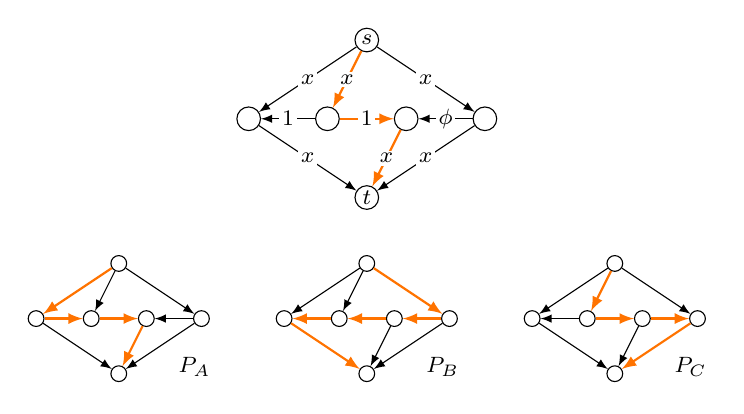
\begin{tikzpicture}[
  font=\footnotesize,
  scale=0.5,
  node/.style={circle, draw, minimum size=3mm, inner sep=0pt},
  smallnode/.style={circle, draw, minimum size=2mm, inner sep=0pt},
  edge/.style={-latex},
  path/.style={-latex, thick, draw=orange!90!red},
  lbl/.style={midway, fill=white, inner sep=1pt}
]

%======================
% TOP NETWORK + PATH
%======================

% nodes
\node[node] (s) at (0,2) {$s$};
\node[node] (a) at (-3,0) {};
\node[node] (u) at (-1,0) {};
\node[node] (v) at (1,0) {};
\node[node] (b) at (3,0) {};
\node[node] (t) at (0,-2) {$t$};

% % start / sink arrows
% \draw[edge] (0,3) -- (s);
% \draw[edge] (t) -- (0,-3);

% outer black diamond edges
\draw[edge] (s) -- node[lbl] {$x$} (a);
\draw[edge] (s) -- node[lbl] {$x$} (b);
\draw[edge] (a) -- node[lbl] {$x$} (t);
\draw[edge] (b) -- node[lbl] {$x$} (t);

% inner black edges
\draw[edge] (u) -- node[lbl] {$1$} (a);
\draw[edge] (b) -- node[lbl] {$\phi$} (v);

% highlighted orange path (s -> u -> v -> t)
\draw[path] (s) -- node[lbl] {$x$} (u);
\draw[path] (u) -- node[lbl] {$1$} (v);
\draw[path] (v) -- node[lbl] {$x$} (t);

%======================
% HELPER: base graph (no labels)
%======================

\newcommand{\basegraph}[6]{%
  % #1..#6 are node names: S A U V B T

  % nodes
  \node[smallnode] (#1) at (0,2) {};
  \node[smallnode] (#2) at (-3,0) {};
  \node[smallnode] (#3) at (-1,0) {};
  \node[smallnode] (#4) at (1,0) {};
  \node[smallnode] (#5) at (3,0) {};
  \node[smallnode] (#6) at (0,-2) {};

  % % edge
  % \draw[edge] (#1) -- (#2);
  % \draw[edge] (#1) -- (#5);
  % \draw[edge] (#2) -- (#6);
  % \draw[edge] (#5) -- (#6);

  % \draw[edge] (#3) -- (#2);
  % \draw[edge] (#5) -- (#4);
  % \draw[edge] (#1) -- (#3);
  % \draw[edge] (#3) -- (#4);
  % \draw[edge] (#4) -- (#6);
}

%======================
% BOTTOM: PATH A
%======================

\begin{scope}[scale= 0.7, yshift=-7.25cm, xshift=-9cm]
  \basegraph{sA}{aA}{uA}{vA}{bA}{tA}

  % orange path A: top -> left side -> u -> v -> bottom
  \draw[path] (sA) -- (aA);
  \draw[path] (aA) -- (uA);
  \draw[path] (uA) -- (vA);
  \draw[path] (vA) -- (tA);

  % other edges
  \draw[edge] (sA) -- (bA);
  \draw[edge] (sA) -- (uA);
  \draw[edge] (bA) -- (vA);
  \draw[edge] (aA) -- (tA);
  \draw[edge] (bA) -- (tA);

  \node at (2.75,-1.75) {$P_A$};
\end{scope}

%======================
% BOTTOM: PATH B
%======================

\begin{scope}[scale= 0.7, yshift=-7.25cm]
  \basegraph{sB}{aB}{uB}{vB}{bB}{tB}

  % orange path B: top -> right side -> v -> u -> left side -> bottom
  \draw[path] (sB) -- (bB);
  \draw[path] (bB) -- (vB);
  \draw[path] (vB) -- (uB);
  \draw[path] (uB) -- (aB);
  \draw[path] (aB) -- (tB);

  % other edges
  \draw[edge] (sB) -- (aB);
  \draw[edge] (sB) -- (uB);
  \draw[edge] (vB) -- (tB);
  \draw[edge] (bB) -- (tB);

  \node at (2.75,-1.75) {$P_B$};
\end{scope}

%======================
% BOTTOM: PATH C
%======================

\begin{scope}[scale= 0.7, yshift=-7.25cm, xshift=9cm]
  \basegraph{sC}{aC}{uC}{vC}{bC}{tC}

  % orange path C: top -> u -> v -> right side -> bottom
  \draw[path] (sC) -- (uC);
  \draw[path] (uC) -- (vC);
  \draw[path] (vC) -- (bC);
  \draw[path] (bC) -- (tC);

  % other edges
  \draw[edge] (sC) -- (aC);
  \draw[edge] (sC) -- (bC);
  \draw[edge] (uC) -- (aC);
  \draw[edge] (aC) -- (tC);
  \draw[edge] (vC) -- (tC);

  \node at (2.75,-1.75) {$P_C$};
\end{scope}

\end{tikzpicture}
\]
where \(\phi = \frac{\sqrt{5} - 1}{2} \approx 0.618\) denotes the golden ratio, satisfying \(\phi^2 + \phi = 1\).
\end{example}


Goal: Choose augmenting paths so that:
\begin{itemize}
  \item can find augmenting paths efficiently
  \item result in few iterations
\end{itemize}

Strategies:
\begin{itemize}
  \item max bottleneck capacity (dependency on \(C\))
  \item sufficiently large bottleneck capacity (Dinitz 1970). reduce dependency on \(C\) to \(\log C\). Time \(O(m^2 \log C)\).
  \item simple/stupid idea: don't do anything fancy with capacities, just choose the path with fewest number of edges (Edmonds-Karp 1972). Polynomial time algorithm. Time \(O(n m^2)\).
\end{itemize}


\subsubsection{Edmonds-Karp}

\emph{Idea}: Always choose an augmenting path with the \hl{minimum number of edges} in the residual network.

\begin{itemize}
  \item Implemented by running \nameref{alg:bfs} in \(G_f\)
  \item Each augmentation increases the shortest path distance
  \item Total number of iterations: \(O(nm)\), so total running time is \hl[2]{\(O(n m^2)\)}
\end{itemize}


\subsection{Bipartite Matching}\label{sec:bipartite_matching}


\begin{theorem}[Marriage]\label{thm:hall-marriage}
\textcolor{AccentGray}{[Frobenius 1917, Hall 1935]} 
Let \(G = (L \cup R, E)\) be a bipartite graph with \(|L| = |R|\).
Then, \(G\) has a perfect matching iff \(|N(S)| \ge |S|\) for all subsets \(S \subseteq L\).
\end{theorem}



